\documentclass{article}
\usepackage{tikz}

\begin{document}

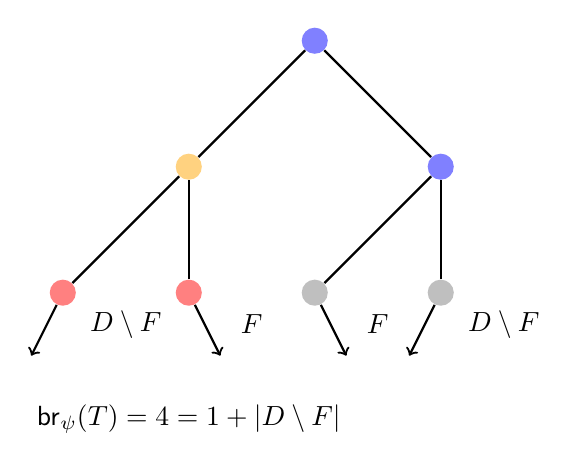
\begin{tikzpicture}[scale=0.8]
    % Define colors
    \definecolor{red}{RGB}{255,0,0}
    \definecolor{orange}{RGB}{255,165,0}
    \definecolor{blue}{RGB}{0,0,255}
    
    % Draw the tree
    \node[circle,fill=blue!50] (root) at (0,0) {};
    \node[circle,fill=orange!50] (left-child) at (-2,-2) {};
    \node[circle,fill=red!50] (left-left-grandchild) at (-4,-4) {};
    \node[circle,fill=red!50] (left-right-grandchild) at (-2,-4) {};
    \node[circle,fill=blue!50] (right-child) at (2,-2) {};
    \node[circle,fill=gray!50] (right-left-grandchild) at (0,-4) {};
    \node[circle,fill=gray!50] (right-right-grandchild) at (2,-4) {};
    
    % Draw the edges
    \draw[thick] (root) -- (left-child);
    \draw[thick] (root) -- (right-child);
    \draw[thick] (left-child) -- (left-left-grandchild);
    \draw[thick] (left-child) -- (left-right-grandchild);
    \draw[thick] (right-child) -- (right-left-grandchild);
    \draw[thick] (right-child) -- (right-right-grandchild);
    
    % Draw the arrows
    \draw[->, thick] (left-left-grandchild) -- ++(-0.5,-1);
    \draw[->, thick] (left-right-grandchild) -- ++(0.5,-1);
    \draw[->, thick] (right-left-grandchild) -- ++(0.5,-1);
    \draw[->, thick] (right-right-grandchild) -- ++(-0.5,-1);
    
    % Add labels
    \node at (-3,-4.5) {$D \setminus F$};
    \node at (-1,-4.5) {$F$};
    \node at (1,-4.5) {$F$};
    \node at (3,-4.5) {$D \setminus F$};
    
    % Add text for the definition
    \node at (-2,-6) {$\mathsf{br}_\psi(T) = 4 = 1 + |D \setminus F|$};
\end{tikzpicture}

\end{document}